\begin{longtable}{|r l p{5cm}|p{3cm}|}
\hline
\multicolumn{3}{|c|}{Fonte} & Requisito\tabularnewline
\hline
 &  & Capitolato & \hyperlink{R-3V1}{R-3V1}

\hyperlink{R-3V2}{R-3V2}

\hyperlink{R-3V3}{R-3V3}

\hyperlink{R-3V3.1}{R-3V3.1}

\hyperlink{R-3V3.2}{R-3V3.2}

\hyperlink{R-3V4}{R-3V4}

\hyperlink{R-3V3.3}{R-3V3.3}

\hyperlink{R-3V5}{R-3V5}

\hyperlink{R-3V6}{R-3V6}

\hyperlink{R-3V6.1}{R-3V6.1}

\hyperlink{R-3V6.2}{R-3V6.2}

\hyperlink{R-3F7.1}{R-3F7.1}

\hyperlink{R-3F7.5.1}{R-3F7.5.1}

\hyperlink{R-3F7.2}{R-3F7.2}

\hyperlink{R-3F7.3}{R-3F7.3}

\hyperlink{R-2F7.5.2}{R-2F7.5.2}

\hyperlink{R-3F7.4}{R-3F7.4}

\hyperlink{R-3F7.5}{R-3F7.5}

\hyperlink{R-3F7}{R-3F7}

\hyperlink{R-3F7.7}{R-3F7.7}

\hyperlink{R-3F9}{R-3F9}

\hyperlink{R-3F10}{R-3F10}

\hyperlink{R-3V12}{R-3V12}

\hyperlink{R-3V3.4}{R-3V3.4}

\hyperlink{R-2F7.8}{R-2F7.8}

\hyperlink{R-2F7.9}{R-2F7.9}

\hyperlink{R-3F7.10}{R-3F7.10}

\hyperlink{R-3F7.10.1}{R-3F7.10.1}

\hyperlink{R-3F7.10.2}{R-3F7.10.2}

\hyperlink{R-2F7.10.3}{R-2F7.10.3}

\hyperlink{R-3F7.5.5}{R-3F7.5.5}

\hyperlink{R-3F7.5.1.2}{R-3F7.5.1.2}\tabularnewline
\hline
 &  & Proponente & \hyperlink{R-3F7.5.3}{R-3F7.5.3}

\hyperlink{R-2F7.5.4}{R-2F7.5.4}

\hyperlink{R-2F7.6}{R-2F7.6}\tabularnewline
\hline
 &  & Committente & \tabularnewline
\hline
 &  & Interno & \hyperlink{R-3F11.1}{R-3F11.1}

\hyperlink{R-3Q27}{R-3Q27}

\hyperlink{R-3Q28}{R-3Q28}

\hyperlink{R-3Q29}{R-3Q29}

\hyperlink{R-2Q30}{R-2Q30}\tabularnewline
\hline
 & \hyperlink{UC1}{UC1} & \hyperlink{UC1}{Autenticazione} & \hyperlink{R-3F8}{R-3F8}

\hyperlink{R-3F8.1}{R-3F8.1}

\hyperlink{R-3F8.2}{R-3F8.2}\tabularnewline
\hline
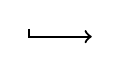
\begin{tikzpicture}
\draw [->, thick] (0.2,0.2) -- (0.2,0.1) -- (1,0.1);
\end{tikzpicture} & \hyperlink{UC1.1}{UC1.1} & \hyperlink{UC1.1}{Registrazione} & \hyperlink{R-3F11}{R-3F11}

\hyperlink{R-3F11.2}{R-3F11.2}

\hyperlink{R-3F11.2.1}{R-3F11.2.1}

\hyperlink{R-3F11.2.2}{R-3F11.2.2}

\hyperlink{R-3F11.2.3}{R-3F11.2.3}

\hyperlink{R-3F11.4}{R-3F11.4}

\hyperlink{R-3F11.4.1}{R-3F11.4.1}

\hyperlink{R-3F11.4.2}{R-3F11.4.2}

\hyperlink{R-3F11.4.3}{R-3F11.4.3}

\hyperlink{R-3F11.2.4}{R-3F11.2.4}

\hyperlink{R-3F11.2.1.1}{R-3F11.2.1.1}

\hyperlink{R-3F11.2.1.2}{R-3F11.2.1.2}

\hyperlink{R-3F11.2.5}{R-3F11.2.5}

\hyperlink{R-3F11.2.1.3}{R-3F11.2.1.3}

\hyperlink{R-3F11.2.1.2.1}{R-3F11.2.1.2.1}\tabularnewline
\hline
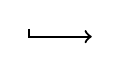
\begin{tikzpicture}
\draw [->, thick] (0.2,0.2) -- (0.2,0.1) -- (1,0.1);
\end{tikzpicture} & \hyperlink{UC1.2}{UC1.2} & \hyperlink{UC1.2}{Errore autenticazione annullata} & \tabularnewline
\hline
 & \hyperlink{UC5}{UC5} & \hyperlink{UC5}{Gestione account} & \hyperlink{R-3F15}{R-3F15}

\hyperlink{R-3F15.1}{R-3F15.1}

\hyperlink{R-3F15.2}{R-3F15.2}

\hyperlink{R-3F15.1.1}{R-3F15.1.1}

\hyperlink{R-3F15.2.1}{R-3F15.2.1}

\hyperlink{R-3F15.3}{R-3F15.3}

\hyperlink{R-3F15.3.1}{R-3F15.3.1}

\hyperlink{R-3F15.3.2}{R-3F15.3.2}

\hyperlink{R-3F15.2.1.1}{R-3F15.2.1.1}

\hyperlink{R-3F15.2.2}{R-3F15.2.2}

\hyperlink{R-3F15.2.2.1}{R-3F15.2.2.1}

\hyperlink{R-3F15.2.2.2}{R-3F15.2.2.2}

\hyperlink{R-3F15.3.3}{R-3F15.3.3}

\hyperlink{R-3F15.1.2}{R-3F15.1.2}\tabularnewline
\hline
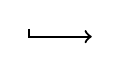
\begin{tikzpicture}
\draw [->, thick] (0.2,0.2) -- (0.2,0.1) -- (1,0.1);
\end{tikzpicture} & \hyperlink{UC5.1}{UC5.1} & \hyperlink{UC5.1}{Modifica informazioni personali} & \hyperlink{R-3F15.3}{R-3F15.3}

\hyperlink{R-3F15.3.1}{R-3F15.3.1}

\hyperlink{R-3F15.3.2}{R-3F15.3.2}

\hyperlink{R-3F15.3.3}{R-3F15.3.3}\tabularnewline
\hline
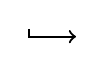
\begin{tikzpicture}
\draw [->, thick] (0.4,0.2) -- (0.4,0.1) -- (1,0.1);
\end{tikzpicture} & \hyperlink{UC5.1.1}{UC5.1.1} & \hyperlink{UC5.1.1}{Modifica nome} & \hyperlink{R-3F15.3.1}{R-3F15.3.1}

\hyperlink{R-3F15.3.3}{R-3F15.3.3}\tabularnewline
\hline
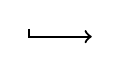
\begin{tikzpicture}
\draw [->, thick] (0.2,0.2) -- (0.2,0.1) -- (1,0.1);
\end{tikzpicture} & \hyperlink{UC5.2}{UC5.2} & \hyperlink{UC5.2}{Errore cancellazione campi obbligatori} & \hyperlink{R-3F15.3.3}{R-3F15.3.3}\tabularnewline
\hline
 & \hyperlink{UC6}{UC6} & \hyperlink{UC6}{Logout} & \hyperlink{R-3F19}{R-3F19}\tabularnewline
\hline
 & \hyperlink{UC7}{UC7} & \hyperlink{UC7}{Gestione domande} & \hyperlink{R-3F7.11}{R-3F7.11}

\hyperlink{R-3F7.11.1}{R-3F7.11.1}

\hyperlink{R-3F7.11.2}{R-3F7.11.2}

\hyperlink{R-3F7.11.3}{R-3F7.11.3}

\hyperlink{R-3F7.11.1.1}{R-3F7.11.1.1}

\hyperlink{R-3F7.11.1.2}{R-3F7.11.1.2}

\hyperlink{R-3F7.11.1.1.1}{R-3F7.11.1.1.1}

\hyperlink{R-3F7.11.1.2.1}{R-3F7.11.1.2.1}\tabularnewline
\hline
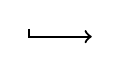
\begin{tikzpicture}
\draw [->, thick] (0.2,0.2) -- (0.2,0.1) -- (1,0.1);
\end{tikzpicture} & \hyperlink{UC7.1}{UC7.1} & \hyperlink{UC7.1}{Inserimento domanda} & \hyperlink{R-2F7.5.2}{R-2F7.5.2}

\hyperlink{R-3F7.5.3}{R-3F7.5.3}

\hyperlink{R-3F7.11.1}{R-3F7.11.1}

\hyperlink{R-3F7.11.1.1}{R-3F7.11.1.1}

\hyperlink{R-3F7.11.1.2.2}{R-3F7.11.1.2.2}

\hyperlink{R-3F7.11.1.2.3}{R-3F7.11.1.2.3}

\hyperlink{R-3F7.11.1.2.4}{R-3F7.11.1.2.4}

\hyperlink{R-2F7.11.1.2.5}{R-2F7.11.1.2.5}

\hyperlink{R-2F7.11.1.2.6}{R-2F7.11.1.2.6}

\hyperlink{R-2F7.11.1.2.7}{R-2F7.11.1.2.7}

\hyperlink{R-3F7.5.5}{R-3F7.5.5}\tabularnewline
\hline
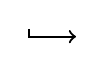
\begin{tikzpicture}
\draw [->, thick] (0.4,0.2) -- (0.4,0.1) -- (1,0.1);
\end{tikzpicture} & \hyperlink{UC7.1.1}{UC7.1.1} & \hyperlink{UC7.1.1}{Selezione argomenti nuova domanda} & \hyperlink{R-3F7.11.1.1}{R-3F7.11.1.1}

\hyperlink{R-3F7.11.1.1.1}{R-3F7.11.1.1.1}\tabularnewline
\hline
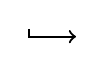
\begin{tikzpicture}
\draw [->, thick] (0.4,0.2) -- (0.4,0.1) -- (1,0.1);
\end{tikzpicture} & \hyperlink{UC7.1.2}{UC7.1.2} & \hyperlink{UC7.1.2}{Scrittura domanda in QML della nuova domanda} & \hyperlink{R-3F7.5.1}{R-3F7.5.1}

\hyperlink{R-3F7.5}{R-3F7.5}

\hyperlink{R-3F7.11.1.2}{R-3F7.11.1.2}

\hyperlink{R-3F7.11.1.2.1}{R-3F7.11.1.2.1}

\hyperlink{R-2F7.5.1.1}{R-2F7.5.1.1}

\hyperlink{R-3F7.5.1.2}{R-3F7.5.1.2}

\hyperlink{R-2F7.5.1.3}{R-2F7.5.1.3}

\hyperlink{R-2F7.5.1.4}{R-2F7.5.1.4}

\hyperlink{R-3F7.5.1.5}{R-3F7.5.1.5}

\hyperlink{R-3F7.5.1.6}{R-3F7.5.1.6}

\hyperlink{R-2F7.5.1.7}{R-2F7.5.1.7}

\hyperlink{R-2F7.5.1.8}{R-2F7.5.1.8}\tabularnewline
\hline
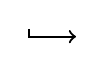
\begin{tikzpicture}
\draw [->, thick] (0.4,0.2) -- (0.4,0.1) -- (1,0.1);
\end{tikzpicture} & \hyperlink{UC7.1.3}{UC7.1.3} & \hyperlink{UC7.1.3}{Scrittura nuova domanda da interfaccia grafica} & \hyperlink{R-2F7.5.4}{R-2F7.5.4}

\hyperlink{R-2F7.5.1.7}{R-2F7.5.1.7}

\hyperlink{R-2F7.5.1.8}{R-2F7.5.1.8}\tabularnewline
\hline
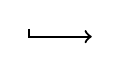
\begin{tikzpicture}
\draw [->, thick] (0.2,0.2) -- (0.2,0.1) -- (1,0.1);
\end{tikzpicture} & \hyperlink{UC7.2}{UC7.2} & \hyperlink{UC7.2}{Modifica domanda} & \hyperlink{R-3F7.11.2}{R-3F7.11.2}\tabularnewline
\hline
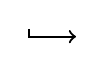
\begin{tikzpicture}
\draw [->, thick] (0.4,0.2) -- (0.4,0.1) -- (1,0.1);
\end{tikzpicture} & \hyperlink{UC7.2.1}{UC7.2.1} & \hyperlink{UC7.2.1}{Selezione argomenti modifica domanda} & \tabularnewline
\hline
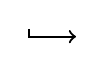
\begin{tikzpicture}
\draw [->, thick] (0.4,0.2) -- (0.4,0.1) -- (1,0.1);
\end{tikzpicture} & \hyperlink{UC7.2.2}{UC7.2.2} & \hyperlink{UC7.2.2}{Scrittura domanda in QML della domanda da modificare} & \tabularnewline
\hline
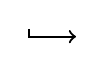
\begin{tikzpicture}
\draw [->, thick] (0.4,0.2) -- (0.4,0.1) -- (1,0.1);
\end{tikzpicture} & \hyperlink{UC7.2.3}{UC7.2.3} & \hyperlink{UC7.2.3}{Modifica domanda da interfaccia grafica} & \tabularnewline
\hline
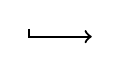
\begin{tikzpicture}
\draw [->, thick] (0.2,0.2) -- (0.2,0.1) -- (1,0.1);
\end{tikzpicture} & \hyperlink{UC7.3}{UC7.3} & \hyperlink{UC7.3}{Elimina domanda} & \hyperlink{R-3F7.11.3}{R-3F7.11.3}\tabularnewline
\hline
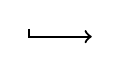
\begin{tikzpicture}
\draw [->, thick] (0.2,0.2) -- (0.2,0.1) -- (1,0.1);
\end{tikzpicture} & \hyperlink{UC7.4}{UC7.4} & \hyperlink{UC7.4}{Errore QML non valido} & \hyperlink{R-3F7.11.1.2.1}{R-3F7.11.1.2.1}\tabularnewline
\hline
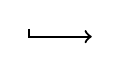
\begin{tikzpicture}
\draw [->, thick] (0.2,0.2) -- (0.2,0.1) -- (1,0.1);
\end{tikzpicture} & \hyperlink{UC7.5}{UC7.5} & \hyperlink{UC7.5}{Errore argomento mancante} & \hyperlink{R-3F7.11.1.1.1}{R-3F7.11.1.1.1}\tabularnewline
\hline
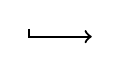
\begin{tikzpicture}
\draw [->, thick] (0.2,0.2) -- (0.2,0.1) -- (1,0.1);
\end{tikzpicture} & \hyperlink{UC7.6}{UC7.6} & \hyperlink{UC7.6}{Inserimento domanda di tipo vero/falso} & \hyperlink{R-3F7.11.1.2.2}{R-3F7.11.1.2.2}

\hyperlink{R-3F7.5.5}{R-3F7.5.5}\tabularnewline
\hline
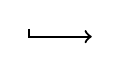
\begin{tikzpicture}
\draw [->, thick] (0.2,0.2) -- (0.2,0.1) -- (1,0.1);
\end{tikzpicture} & \hyperlink{UC7.7}{UC7.7} & \hyperlink{UC7.7}{Inserimento domanda a scelta multipla} & \hyperlink{R-3F7.11.1.2.3}{R-3F7.11.1.2.3}\tabularnewline
\hline
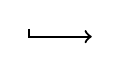
\begin{tikzpicture}
\draw [->, thick] (0.2,0.2) -- (0.2,0.1) -- (1,0.1);
\end{tikzpicture} & \hyperlink{UC7.8}{UC7.8} & \hyperlink{UC7.8}{Inserimento domanda a risposta multipla} & \hyperlink{R-2F7.5.2}{R-2F7.5.2}

\hyperlink{R-3F7.11.1.2.4}{R-3F7.11.1.2.4}

\hyperlink{R-3F7.5.5}{R-3F7.5.5}\tabularnewline
\hline
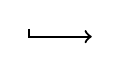
\begin{tikzpicture}
\draw [->, thick] (0.2,0.2) -- (0.2,0.1) -- (1,0.1);
\end{tikzpicture} & \hyperlink{UC7.9}{UC7.9} & \hyperlink{UC7.9}{Inserimento domanda di tipo testo con parole omesse} & \hyperlink{R-2F7.5.2}{R-2F7.5.2}

\hyperlink{R-2F7.11.1.2.5}{R-2F7.11.1.2.5}\tabularnewline
\hline
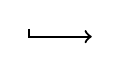
\begin{tikzpicture}
\draw [->, thick] (0.2,0.2) -- (0.2,0.1) -- (1,0.1);
\end{tikzpicture} & \hyperlink{UC7.10}{UC7.10} & \hyperlink{UC7.10}{Inserimento domanda con l'associazione di parole} & \hyperlink{R-2F7.5.2}{R-2F7.5.2}

\hyperlink{R-2F7.11.1.2.6}{R-2F7.11.1.2.6}\tabularnewline
\hline
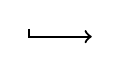
\begin{tikzpicture}
\draw [->, thick] (0.2,0.2) -- (0.2,0.1) -- (1,0.1);
\end{tikzpicture} & \hyperlink{UC7.11}{UC7.11} & \hyperlink{UC7.11}{Inserimento domanda a risposta aperta} & \hyperlink{R-2F7.5.2}{R-2F7.5.2}

\hyperlink{R-2F7.11.1.2.7}{R-2F7.11.1.2.7}\tabularnewline
\hline
 & \hyperlink{UC8}{UC8} & \hyperlink{UC8}{Gestione questionari} & \hyperlink{R-3F7}{R-3F7}

\hyperlink{R-3F7.7}{R-3F7.7}

\hyperlink{R-3F7.11}{R-3F7.11}

\hyperlink{R-3F7.12}{R-3F7.12}

\hyperlink{R-3F7.12.2}{R-3F7.12.2}

\hyperlink{R-3F7.12.3}{R-3F7.12.3}

\hyperlink{R-3F7.13}{R-3F7.13}

\hyperlink{R-3F7.12.4}{R-3F7.12.4}

\hyperlink{R-3F7.7.1}{R-3F7.7.1}\tabularnewline
\hline
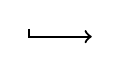
\begin{tikzpicture}
\draw [->, thick] (0.2,0.2) -- (0.2,0.1) -- (1,0.1);
\end{tikzpicture} & \hyperlink{UC8.1}{UC8.1} & \hyperlink{UC8.1}{Inserisci questionario} & \hyperlink{R-3F7.7}{R-3F7.7}

\hyperlink{R-3F7.7.1}{R-3F7.7.1}\tabularnewline
\hline
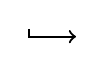
\begin{tikzpicture}
\draw [->, thick] (0.4,0.2) -- (0.4,0.1) -- (1,0.1);
\end{tikzpicture} & \hyperlink{UC8.1.1}{UC8.1.1} & \hyperlink{UC8.1.1}{Aggiungi domanda in un nuovo questionario } & \hyperlink{R-3F7.11}{R-3F7.11}

\hyperlink{R-3F7.12.2}{R-3F7.12.2}

\hyperlink{R-3F7.11.1.2}{R-3F7.11.1.2}

\hyperlink{R-3F7.11.1.1.1}{R-3F7.11.1.1.1}

\hyperlink{R-3F7.11.1.2.1}{R-3F7.11.1.2.1}\tabularnewline
\hline
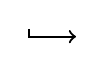
\begin{tikzpicture}
\draw [->, thick] (0.4,0.2) -- (0.4,0.1) -- (1,0.1);
\end{tikzpicture} & \hyperlink{UC8.1.2}{UC8.1.2} & \hyperlink{UC8.1.2}{Elimina domanda da un nuovo questionario} & \hyperlink{R-3F7.11}{R-3F7.11}

\hyperlink{R-3F7.12.3}{R-3F7.12.3}\tabularnewline
\hline
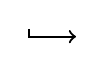
\begin{tikzpicture}
\draw [->, thick] (0.4,0.2) -- (0.4,0.1) -- (1,0.1);
\end{tikzpicture} & \hyperlink{UC8.1.3}{UC8.1.3} & \hyperlink{UC8.1.3}{Seleziona argomenti del nuovo questionario} & \hyperlink{R-3F7.12.4}{R-3F7.12.4}\tabularnewline
\hline
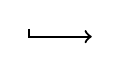
\begin{tikzpicture}
\draw [->, thick] (0.2,0.2) -- (0.2,0.1) -- (1,0.1);
\end{tikzpicture} & \hyperlink{UC8.2}{UC8.2} & \hyperlink{UC8.2}{Modifica questionario} & \hyperlink{R-3F7.12}{R-3F7.12}

\hyperlink{R-3F7.12.4}{R-3F7.12.4}\tabularnewline
\hline
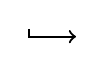
\begin{tikzpicture}
\draw [->, thick] (0.4,0.2) -- (0.4,0.1) -- (1,0.1);
\end{tikzpicture} & \hyperlink{UC8.2.1}{UC8.2.1} & \hyperlink{UC8.2.1}{Aggiungi domanda in un questionario} & \tabularnewline
\hline
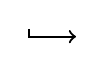
\begin{tikzpicture}
\draw [->, thick] (0.4,0.2) -- (0.4,0.1) -- (1,0.1);
\end{tikzpicture} & \hyperlink{UC8.2.2}{UC8.2.2} & \hyperlink{UC8.2.2}{Elimina domanda da un questionario da  modificare} & \tabularnewline
\hline
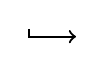
\begin{tikzpicture}
\draw [->, thick] (0.4,0.2) -- (0.4,0.1) -- (1,0.1);
\end{tikzpicture} & \hyperlink{UC8.2.3}{UC8.2.3} & \hyperlink{UC8.2.3}{Selezione argomenti modifica questionario} & \tabularnewline
\hline
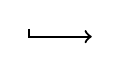
\begin{tikzpicture}
\draw [->, thick] (0.2,0.2) -- (0.2,0.1) -- (1,0.1);
\end{tikzpicture} & \hyperlink{UC8.3}{UC8.3} & \hyperlink{UC8.3}{Elimina questionario} & \hyperlink{R-3F7.13}{R-3F7.13}\tabularnewline
\hline
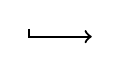
\begin{tikzpicture}
\draw [->, thick] (0.2,0.2) -- (0.2,0.1) -- (1,0.1);
\end{tikzpicture} & \hyperlink{UC8.4}{UC8.4} & \hyperlink{UC8.4}{Errore questionario vuoto} & \hyperlink{R-3F7.7.1}{R-3F7.7.1}\tabularnewline
\hline
 & \hyperlink{UC9}{UC9} & \hyperlink{UC9}{Gestione classi} & \hyperlink{R-2F14.1.1}{R-2F14.1.1}

\hyperlink{R-2F14}{R-2F14}

\hyperlink{R-2F14.1}{R-2F14.1}

\hyperlink{R-2F14.2}{R-2F14.2}

\hyperlink{R-2F14.3}{R-2F14.3}

\hyperlink{R-2F14.1.2}{R-2F14.1.2}

\hyperlink{R-2F14.1.3}{R-2F14.1.3}

\hyperlink{R-2F14.3.1}{R-2F14.3.1}

\hyperlink{R-2F14.3.2}{R-2F14.3.2}

\hyperlink{R-2F14.3.3}{R-2F14.3.3}

\hyperlink{R-2F14.1.1.1}{R-2F14.1.1.1}\tabularnewline
\hline
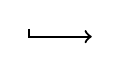
\begin{tikzpicture}
\draw [->, thick] (0.2,0.2) -- (0.2,0.1) -- (1,0.1);
\end{tikzpicture} & \hyperlink{UC9.1}{UC9.1} & \hyperlink{UC9.1}{Inserisci classe} & \hyperlink{R-2F7.6}{R-2F7.6}

\hyperlink{R-2F14.1.1}{R-2F14.1.1}

\hyperlink{R-2F14.1}{R-2F14.1}

\hyperlink{R-2F14.1.2}{R-2F14.1.2}

\hyperlink{R-2F14.1.3}{R-2F14.1.3}

\hyperlink{R-2F14.1.1.1}{R-2F14.1.1.1}\tabularnewline
\hline
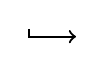
\begin{tikzpicture}
\draw [->, thick] (0.4,0.2) -- (0.4,0.1) -- (1,0.1);
\end{tikzpicture} & \hyperlink{UC9.1.1}{UC9.1.1} & \hyperlink{UC9.1.1}{Inserisci nome classe} & \hyperlink{R-2F14.1.1}{R-2F14.1.1}

\hyperlink{R-2F14.3.1}{R-2F14.3.1}

\hyperlink{R-2F14.1.1.1}{R-2F14.1.1.1}\tabularnewline
\hline
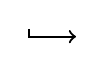
\begin{tikzpicture}
\draw [->, thick] (0.4,0.2) -- (0.4,0.1) -- (1,0.1);
\end{tikzpicture} & \hyperlink{UC9.1.2}{UC9.1.2} & \hyperlink{UC9.1.2}{Inserisci argomenti classe} & \hyperlink{R-2F14.1.2}{R-2F14.1.2}

\hyperlink{R-2F14.3.2}{R-2F14.3.2}\tabularnewline
\hline
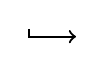
\begin{tikzpicture}
\draw [->, thick] (0.4,0.2) -- (0.4,0.1) -- (1,0.1);
\end{tikzpicture} & \hyperlink{UC9.1.3}{UC9.1.3} & \hyperlink{UC9.1.3}{Inserisci password classe} & \hyperlink{R-2F14.1.3}{R-2F14.1.3}

\hyperlink{R-2F14.3.3}{R-2F14.3.3}\tabularnewline
\hline
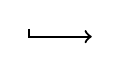
\begin{tikzpicture}
\draw [->, thick] (0.2,0.2) -- (0.2,0.1) -- (1,0.1);
\end{tikzpicture} & \hyperlink{UC9.2}{UC9.2} & \hyperlink{UC9.2}{Modifica classe} & \hyperlink{R-2F14.3}{R-2F14.3}

\hyperlink{R-2F14.3.1}{R-2F14.3.1}

\hyperlink{R-2F14.3.2}{R-2F14.3.2}

\hyperlink{R-2F14.3.3}{R-2F14.3.3}\tabularnewline
\hline
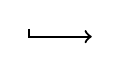
\begin{tikzpicture}
\draw [->, thick] (0.2,0.2) -- (0.2,0.1) -- (1,0.1);
\end{tikzpicture} & \hyperlink{UC9.3}{UC9.3} & \hyperlink{UC9.3}{Elimina classe} & \hyperlink{R-2F14.2}{R-2F14.2}\tabularnewline
\hline
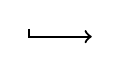
\begin{tikzpicture}
\draw [->, thick] (0.2,0.2) -- (0.2,0.1) -- (1,0.1);
\end{tikzpicture} & \hyperlink{UC9.4}{UC9.4} & \hyperlink{UC9.4}{Errore nome classe già presente} & \hyperlink{R-2F14.1.1.1}{R-2F14.1.1.1}\tabularnewline
\hline
 & \hyperlink{UC10}{UC10} & \hyperlink{UC10}{Gestione argomenti} & \hyperlink{R-3F24}{R-3F24}

\hyperlink{R-3F24.1}{R-3F24.1}

\hyperlink{R-3F24.2}{R-3F24.2}

\hyperlink{R-3F24.3}{R-3F24.3}

\hyperlink{R-3F24.4}{R-3F24.4}

\hyperlink{R-3F24.1.1}{R-3F24.1.1}

\hyperlink{R-3F24.2.1}{R-3F24.2.1}

\hyperlink{R-3F24.2.2}{R-3F24.2.2}\tabularnewline
\hline
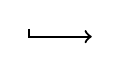
\begin{tikzpicture}
\draw [->, thick] (0.2,0.2) -- (0.2,0.1) -- (1,0.1);
\end{tikzpicture} & \hyperlink{UC10.1}{UC10.1} & \hyperlink{UC10.1}{Esplorazione argomenti} & \hyperlink{R-3F24.4}{R-3F24.4}

\hyperlink{R-3F24.2.1}{R-3F24.2.1}\tabularnewline
\hline
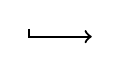
\begin{tikzpicture}
\draw [->, thick] (0.2,0.2) -- (0.2,0.1) -- (1,0.1);
\end{tikzpicture} & \hyperlink{UC10.2}{UC10.2} & \hyperlink{UC10.2}{Crea argomento} & \hyperlink{R-3F24.1}{R-3F24.1}

\hyperlink{R-3F24.1.1}{R-3F24.1.1}\tabularnewline
\hline
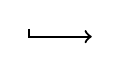
\begin{tikzpicture}
\draw [->, thick] (0.2,0.2) -- (0.2,0.1) -- (1,0.1);
\end{tikzpicture} & \hyperlink{UC10.3}{UC10.3} & \hyperlink{UC10.3}{Argomento già presente nel sistema} & \hyperlink{R-3F24.1.1}{R-3F24.1.1}\tabularnewline
\hline
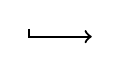
\begin{tikzpicture}
\draw [->, thick] (0.2,0.2) -- (0.2,0.1) -- (1,0.1);
\end{tikzpicture} & \hyperlink{UC10.4}{UC10.4} & \hyperlink{UC10.4}{Modifica argomento} & \hyperlink{R-3F24.3}{R-3F24.3}\tabularnewline
\hline
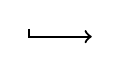
\begin{tikzpicture}
\draw [->, thick] (0.2,0.2) -- (0.2,0.1) -- (1,0.1);
\end{tikzpicture} & \hyperlink{UC10.5}{UC10.5} & \hyperlink{UC10.5}{Eliminazione argomento} & \hyperlink{R-3F24.2}{R-3F24.2}

\hyperlink{R-3F24.2.1}{R-3F24.2.1}

\hyperlink{R-3F24.2.2}{R-3F24.2.2}\tabularnewline
\hline
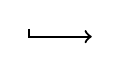
\begin{tikzpicture}
\draw [->, thick] (0.2,0.2) -- (0.2,0.1) -- (1,0.1);
\end{tikzpicture} & \hyperlink{UC10.6}{UC10.6} & \hyperlink{UC10.6}{Errore l'argomento ha domande o questionari} & \hyperlink{R-3F24.2.2}{R-3F24.2.2}\tabularnewline
\hline
 & \hyperlink{UC11}{UC11} & \hyperlink{UC11}{Visualizza statistiche} & \hyperlink{R-2F25.3.1}{R-2F25.3.1}

\hyperlink{R-3F25}{R-3F25}

\hyperlink{R-3F25.1}{R-3F25.1}

\hyperlink{R-3F25.2}{R-3F25.2}

\hyperlink{R-2F25.3}{R-2F25.3}

\hyperlink{R-3F25.1.1}{R-3F25.1.1}

\hyperlink{R-3F25.2.1}{R-3F25.2.1}

\hyperlink{R-2F25.3.2}{R-2F25.3.2}

\hyperlink{R-2F25.3.3}{R-2F25.3.3}

\hyperlink{R-2F25.3.4}{R-2F25.3.4}

\hyperlink{R-3F25.3.4.1}{R-3F25.3.4.1}

\hyperlink{R-2F25.3.5}{R-2F25.3.5}

\hyperlink{R-2F25.3.5.1}{R-2F25.3.5.1}\tabularnewline
\hline
 & \hyperlink{UC12}{UC12} & \hyperlink{UC12}{Visualizza statistiche domanda} & \hyperlink{R-3F25.1}{R-3F25.1}

\hyperlink{R-3F25.1.1}{R-3F25.1.1}\tabularnewline
\hline
 & \hyperlink{UC13}{UC13} & \hyperlink{UC13}{Visualizza statistiche questionario} & \hyperlink{R-3F25.2}{R-3F25.2}

\hyperlink{R-3F25.2.1}{R-3F25.2.1}\tabularnewline
\hline
 & \hyperlink{UC14}{UC14} & \hyperlink{UC14}{Visualizza statistiche classe} & \hyperlink{R-2F25.3.1}{R-2F25.3.1}

\hyperlink{R-2F25.3}{R-2F25.3}

\hyperlink{R-2F25.3.2}{R-2F25.3.2}

\hyperlink{R-2F25.3.3}{R-2F25.3.3}

\hyperlink{R-2F25.3.4}{R-2F25.3.4}

\hyperlink{R-3F25.3.4.1}{R-3F25.3.4.1}

\hyperlink{R-2F25.3.5}{R-2F25.3.5}

\hyperlink{R-2F25.3.5.1}{R-2F25.3.5.1}\tabularnewline
\hline
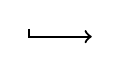
\begin{tikzpicture}
\draw [->, thick] (0.2,0.2) -- (0.2,0.1) -- (1,0.1);
\end{tikzpicture} & \hyperlink{UC14.1}{UC14.1} & \hyperlink{UC14.1}{Visualizza risultati domande della classe} & \hyperlink{R-2F25.3.5}{R-2F25.3.5}

\hyperlink{R-2F25.3.5.1}{R-2F25.3.5.1}\tabularnewline
\hline
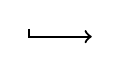
\begin{tikzpicture}
\draw [->, thick] (0.2,0.2) -- (0.2,0.1) -- (1,0.1);
\end{tikzpicture} & \hyperlink{UC14.2}{UC14.2} & \hyperlink{UC14.2}{Visualizza risultati questionari della classe} & \hyperlink{R-2F25.3.1}{R-2F25.3.1}\tabularnewline
\hline
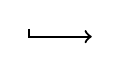
\begin{tikzpicture}
\draw [->, thick] (0.2,0.2) -- (0.2,0.1) -- (1,0.1);
\end{tikzpicture} & \hyperlink{UC14.3}{UC14.3} & \hyperlink{UC14.3}{Visualizza sommario statistiche classe} & \hyperlink{R-2F25.3.3}{R-2F25.3.3}\tabularnewline
\hline
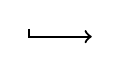
\begin{tikzpicture}
\draw [->, thick] (0.2,0.2) -- (0.2,0.1) -- (1,0.1);
\end{tikzpicture} & \hyperlink{UC14.4}{UC14.4} & \hyperlink{UC14.4}{Visualizza statistiche studente della classe} & \hyperlink{R-2F25.3.4}{R-2F25.3.4}

\hyperlink{R-3F25.3.4.1}{R-3F25.3.4.1}\tabularnewline
\hline
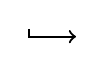
\begin{tikzpicture}
\draw [->, thick] (0.4,0.2) -- (0.4,0.1) -- (1,0.1);
\end{tikzpicture} & \hyperlink{UC14.4.1}{UC14.4.1} & \hyperlink{UC14.4.1}{Visualizza risultati questionari dello studente} & \hyperlink{R-3F25.3.4.1}{R-3F25.3.4.1}\tabularnewline
\hline
 & \hyperlink{UC15}{UC15} & \hyperlink{UC15}{Esegui questionario} & \hyperlink{R-3F18}{R-3F18}

\hyperlink{R-3F18.1}{R-3F18.1}

\hyperlink{R-3F18.2}{R-3F18.2}

\hyperlink{R-3F18.3}{R-3F18.3}

\hyperlink{R-3F18.4}{R-3F18.4}

\hyperlink{R-3F18.2.1}{R-3F18.2.1}\tabularnewline
\hline
\begin{tikzpicture}
\draw [->, thick] (0.2,0.2) -- (0.2,0.1) -- (1,0.1);
\end{tikzpicture} & \hyperlink{UC15.1}{UC15.1} & \hyperlink{UC15.1}{Rispondi domanda} & \hyperlink{R-3F9}{R-3F9}

\hyperlink{R-3F18.1}{R-3F18.1}

\hyperlink{R-3F18.1.1}{R-3F18.1.1}

\hyperlink{R-3F18.1.2}{R-3F18.1.2}

\hyperlink{R-2F18.1.3}{R-2F18.1.3}

\hyperlink{R-2F18.1.4}{R-2F18.1.4}

\hyperlink{R-2F18.1.5}{R-2F18.1.5}

\hyperlink{R-2F18.1.6}{R-2F18.1.6}\tabularnewline
\hline
\begin{tikzpicture}
\draw [->, thick] (0.2,0.2) -- (0.2,0.1) -- (1,0.1);
\end{tikzpicture} & \hyperlink{UC15.2}{UC15.2} & \hyperlink{UC15.2}{Errore domanda non risposta} & \hyperlink{R-3F18.2.1}{R-3F18.2.1}\tabularnewline
\hline
\begin{tikzpicture}
\draw [->, thick] (0.2,0.2) -- (0.2,0.1) -- (1,0.1);
\end{tikzpicture} & \hyperlink{UC15.3}{UC15.3} & \hyperlink{UC15.3}{Conferma questionario} & \hyperlink{R-3F18.2}{R-3F18.2}

\hyperlink{R-3F18.2.1}{R-3F18.2.1}\tabularnewline
\hline
\begin{tikzpicture}
\draw [->, thick] (0.2,0.2) -- (0.2,0.1) -- (1,0.1);
\end{tikzpicture} & \hyperlink{UC15.4}{UC15.4} & \hyperlink{UC15.4}{Rispondi domanda vero/falso} & \hyperlink{R-3F18.1.1}{R-3F18.1.1}\tabularnewline
\hline
\begin{tikzpicture}
\draw [->, thick] (0.2,0.2) -- (0.2,0.1) -- (1,0.1);
\end{tikzpicture} & \hyperlink{UC15.5}{UC15.5} & \hyperlink{UC15.5}{Rispondi domanda a scelta multipla} & \hyperlink{R-3F18.1.2}{R-3F18.1.2}\tabularnewline
\hline
\begin{tikzpicture}
\draw [->, thick] (0.2,0.2) -- (0.2,0.1) -- (1,0.1);
\end{tikzpicture} & \hyperlink{UC15.6}{UC15.6} & \hyperlink{UC15.6}{Rispondi domanda a risposta multipla} & \hyperlink{R-2F18.1.3}{R-2F18.1.3}\tabularnewline
\hline
\begin{tikzpicture}
\draw [->, thick] (0.2,0.2) -- (0.2,0.1) -- (1,0.1);
\end{tikzpicture} & \hyperlink{UC15.7}{UC15.7} & \hyperlink{UC15.7}{Rispondi domanda di tipo testo con parole omesse} & \hyperlink{R-2F18.1.4}{R-2F18.1.4}\tabularnewline
\hline
\begin{tikzpicture}
\draw [->, thick] (0.2,0.2) -- (0.2,0.1) -- (1,0.1);
\end{tikzpicture} & \hyperlink{UC15.8}{UC15.8} & \hyperlink{UC15.8}{Rispondi domanda con associazione di parole} & \hyperlink{R-2F18.1.5}{R-2F18.1.5}\tabularnewline
\hline
\begin{tikzpicture}
\draw [->, thick] (0.2,0.2) -- (0.2,0.1) -- (1,0.1);
\end{tikzpicture} & \hyperlink{UC15.9}{UC15.9} & \hyperlink{UC15.9}{Rispondi domanda a risposta aperta} & \hyperlink{R-2F18.1.6}{R-2F18.1.6}\tabularnewline
\hline
\begin{tikzpicture}
\draw [->, thick] (0.2,0.2) -- (0.2,0.1) -- (1,0.1);
\end{tikzpicture} & \hyperlink{UC15.10}{UC15.10} & \hyperlink{UC15.10}{Feedback questionario} & \hyperlink{R-2F7.9}{R-2F7.9}\tabularnewline
\hline
 & \hyperlink{UC16}{UC16} & \hyperlink{UC16}{Iscrizione ad una classe} & \hyperlink{R-2F7.6}{R-2F7.6}

\hyperlink{R-2F17}{R-2F17}

\hyperlink{R-2F17.1}{R-2F17.1}

\hyperlink{R-2F17.1.1}{R-2F17.1.1}\tabularnewline
\hline
\begin{tikzpicture}
\draw [->, thick] (0.2,0.2) -- (0.2,0.1) -- (1,0.1);
\end{tikzpicture} & \hyperlink{UC16.1}{UC16.1} & \hyperlink{UC16.1}{Inserisci password classe} & \hyperlink{R-2F17.1}{R-2F17.1}\tabularnewline
\hline
\begin{tikzpicture}
\draw [->, thick] (0.2,0.2) -- (0.2,0.1) -- (1,0.1);
\end{tikzpicture} & \hyperlink{UC16.2}{UC16.2} & \hyperlink{UC16.2}{Errore password classe} & \hyperlink{R-2F17.1.1}{R-2F17.1.1}\tabularnewline
\hline
 & \hyperlink{UC17}{UC17} & \hyperlink{UC17}{Visualizza storico studente} & \hyperlink{R-3F7.4}{R-3F7.4}

\hyperlink{R-3F7.10}{R-3F7.10}

\hyperlink{R-3F7.10.1}{R-3F7.10.1}

\hyperlink{R-3F7.10.2}{R-3F7.10.2}

\hyperlink{R-2F7.10.3}{R-2F7.10.3}

\hyperlink{R-3F26}{R-3F26}

\hyperlink{R-3F26.1}{R-3F26.1}

\hyperlink{R-3F26.2}{R-3F26.2}

\hyperlink{R-3F26.3}{R-3F26.3}

\hyperlink{R-3F26.3.1}{R-3F26.3.1}

\hyperlink{R-3F26.1.1}{R-3F26.1.1}

\hyperlink{R-3F26.1.2}{R-3F26.1.2}

\hyperlink{R-3F26.1.3}{R-3F26.1.3}

\hyperlink{R-3F26.1.4}{R-3F26.1.4}

\hyperlink{R-1F26.1.5}{R-1F26.1.5}

\hyperlink{R-3F26.2.1}{R-3F26.2.1}

\hyperlink{R-3F26.2.2}{R-3F26.2.2}

\hyperlink{R-3F26.3.2}{R-3F26.3.2}

\hyperlink{R-3F26.3.3}{R-3F26.3.3}

\hyperlink{R-3F26.3.4}{R-3F26.3.4}\tabularnewline
\hline
\begin{tikzpicture}
\draw [->, thick] (0.2,0.2) -- (0.2,0.1) -- (1,0.1);
\end{tikzpicture} & \hyperlink{UC17.1}{UC17.1} & \hyperlink{UC17.1}{Visualizza statistiche domande studente} & \hyperlink{R-3F26.2}{R-3F26.2}

\hyperlink{R-3F26.2.1}{R-3F26.2.1}

\hyperlink{R-3F26.2.2}{R-3F26.2.2}\tabularnewline
\hline
\begin{tikzpicture}
\draw [->, thick] (0.2,0.2) -- (0.2,0.1) -- (1,0.1);
\end{tikzpicture} & \hyperlink{UC17.2}{UC17.2} & \hyperlink{UC17.2}{Visualizza statistiche questionari studente} & \hyperlink{R-3F7.10.2}{R-3F7.10.2}

\hyperlink{R-3F26.3}{R-3F26.3}

\hyperlink{R-3F26.3.1}{R-3F26.3.1}

\hyperlink{R-3F26.3.2}{R-3F26.3.2}

\hyperlink{R-3F26.3.3}{R-3F26.3.3}

\hyperlink{R-3F26.3.4}{R-3F26.3.4}\tabularnewline
\hline
\begin{tikzpicture}
\draw [->, thick] (0.2,0.2) -- (0.2,0.1) -- (1,0.1);
\end{tikzpicture} & \hyperlink{UC17.3}{UC17.3} & \hyperlink{UC17.3}{Visualizza sommario statistiche studente} & \hyperlink{R-2F7.10.3}{R-2F7.10.3}

\hyperlink{R-3F26.1}{R-3F26.1}

\hyperlink{R-3F26.1.1}{R-3F26.1.1}

\hyperlink{R-3F26.1.2}{R-3F26.1.2}

\hyperlink{R-3F26.1.3}{R-3F26.1.3}

\hyperlink{R-3F26.1.4}{R-3F26.1.4}

\hyperlink{R-1F26.1.5}{R-1F26.1.5}\tabularnewline
\hline
 & \hyperlink{UC18}{UC18} & \hyperlink{UC18}{Ricerca questionario} & \hyperlink{R-3F7.12.1}{R-3F7.12.1}

\hyperlink{R-3F16}{R-3F16}

\hyperlink{R-3F16.1}{R-3F16.1}

\hyperlink{R-2F16.2}{R-2F16.2}

\hyperlink{R-3F16.3}{R-3F16.3}

\hyperlink{R-3F16.4}{R-3F16.4}

\hyperlink{R-3F16.5}{R-3F16.5}

\hyperlink{R-3F25.2.1}{R-3F25.2.1}

\hyperlink{R-3F25.3.4.1}{R-3F25.3.4.1}

\hyperlink{R-3F26.3.1}{R-3F26.3.1}\tabularnewline
\hline
 & \hyperlink{UC19}{UC19} & \hyperlink{UC19}{Ricerca questionario per titolo} & \hyperlink{R-3F16.1}{R-3F16.1}\tabularnewline
\hline
 & \hyperlink{UC20}{UC20} & \hyperlink{UC20}{Ricerca questionario per classe} & \hyperlink{R-2F16.2}{R-2F16.2}\tabularnewline
\hline
 & \hyperlink{UC21}{UC21} & \hyperlink{UC21}{Ricerca questionario per argomento} & \hyperlink{R-3F16.4}{R-3F16.4}\tabularnewline
\hline
 & \hyperlink{UC22}{UC22} & \hyperlink{UC22}{Ricerca questionario per docente} & \hyperlink{R-3F16.3}{R-3F16.3}\tabularnewline
\hline
 & \hyperlink{UC23}{UC23} & \hyperlink{UC23}{Ricerca questionario per difficoltà} & \hyperlink{R-3F16.5}{R-3F16.5}\tabularnewline
\hline
 & \hyperlink{UC24}{UC24} & \hyperlink{UC24}{Ricerca domanda} & \hyperlink{R-3F21}{R-3F21}

\hyperlink{R-3F21.1}{R-3F21.1}

\hyperlink{R-3F21.2}{R-3F21.2}

\hyperlink{R-3F21.3}{R-3F21.3}

\hyperlink{R-3F21.4}{R-3F21.4}

\hyperlink{R-3F25.1.1}{R-3F25.1.1}

\hyperlink{R-2F25.3.5.1}{R-2F25.3.5.1}\tabularnewline
\hline
 & \hyperlink{UC25}{UC25} & \hyperlink{UC25}{Ricerca domanda per keywords} & \hyperlink{R-3F21.4}{R-3F21.4}\tabularnewline
\hline
 & \hyperlink{UC26}{UC26} & \hyperlink{UC26}{Ricerca domanda per argomento} & \hyperlink{R-3F21.1}{R-3F21.1}\tabularnewline
\hline
 & \hyperlink{UC27}{UC27} & \hyperlink{UC27}{Ricerca domanda per difficoltà} & \hyperlink{R-3F21.3}{R-3F21.3}\tabularnewline
\hline
 & \hyperlink{UC28}{UC28} & \hyperlink{UC28}{Ricerca domanda per docente} & \hyperlink{R-3F21.2}{R-3F21.2}\tabularnewline
\hline
 & \hyperlink{UC29}{UC29} & \hyperlink{UC29}{Ricerca classe} & \hyperlink{R-2F17.2}{R-2F17.2}

\hyperlink{R-2F22}{R-2F22}

\hyperlink{R-2F22.1}{R-2F22.1}

\hyperlink{R-2F22.2}{R-2F22.2}\tabularnewline
\hline
 & \hyperlink{UC30}{UC30} & \hyperlink{UC30}{Ricerca classe per docente} & \hyperlink{R-2F17.2}{R-2F17.2}

\hyperlink{R-2F22.2}{R-2F22.2}\tabularnewline
\hline
 & \hyperlink{UC31}{UC31} & \hyperlink{UC31}{Ricerca classe per argomento} & \hyperlink{R-2F17.2}{R-2F17.2}

\hyperlink{R-2F22.1}{R-2F22.1}\tabularnewline
\hline
 & \hyperlink{UC32}{UC32} & \hyperlink{UC32}{Azioni Amministratore} & \hyperlink{R-3F11.3}{R-3F11.3}

\hyperlink{R-3F13}{R-3F13}

\hyperlink{R-3F13.1}{R-3F13.1}

\hyperlink{R-3F13.2}{R-3F13.2}

\hyperlink{R-3F13.3}{R-3F13.3}

\hyperlink{R-3F13.4}{R-3F13.4}\tabularnewline
\hline
\begin{tikzpicture}
\draw [->, thick] (0.2,0.2) -- (0.2,0.1) -- (1,0.1);
\end{tikzpicture} & \hyperlink{UC32.1}{UC32.1} & \hyperlink{UC32.1}{Cambia ruolo} & \hyperlink{R-3F11.3}{R-3F11.3}

\hyperlink{R-3F13.1}{R-3F13.1}

\hyperlink{R-3F13.4}{R-3F13.4}\tabularnewline
\hline
\begin{tikzpicture}
\draw [->, thick] (0.2,0.2) -- (0.2,0.1) -- (1,0.1);
\end{tikzpicture} & \hyperlink{UC32.2}{UC32.2} & \hyperlink{UC32.2}{Rimuovi  docente} & \hyperlink{R-3F13.2}{R-3F13.2}\tabularnewline
\hline
 & \hyperlink{UC33}{UC33} & \hyperlink{UC33}{Azioni proprietario} & \hyperlink{R-3F11.5}{R-3F11.5}

\hyperlink{R-3F20}{R-3F20}

\hyperlink{R-3F20.1}{R-3F20.1}

\hyperlink{R-3F20.2}{R-3F20.2}

\hyperlink{R-3F20.3}{R-3F20.3}

\hyperlink{R-3F20.2.1}{R-3F20.2.1}\tabularnewline
\hline
\begin{tikzpicture}
\draw [->, thick] (0.2,0.2) -- (0.2,0.1) -- (1,0.1);
\end{tikzpicture} & \hyperlink{UC33.1}{UC33.1} & \hyperlink{UC33.1}{Aggiungi amministratore} & \hyperlink{R-3F11.5}{R-3F11.5}

\hyperlink{R-3F20.2}{R-3F20.2}

\hyperlink{R-3F20.2.1}{R-3F20.2.1}\tabularnewline
\hline
\begin{tikzpicture}
\draw [->, thick] (0.2,0.2) -- (0.2,0.1) -- (1,0.1);
\end{tikzpicture} & \hyperlink{UC33.2}{UC33.2} & \hyperlink{UC33.2}{Elimina amministratore} & \hyperlink{R-3F20.3}{R-3F20.3}\tabularnewline
\hline
 & \hyperlink{UC2}{UC2} & \hyperlink{UC2}{Autenticazione con Google} & \tabularnewline
\hline
 & \hyperlink{UC3}{UC3} & \hyperlink{UC3}{Autenticazione con Facebook} & \tabularnewline
\hline
 & \hyperlink{UC4}{UC4} & \hyperlink{UC4}{Autenticazione con Windows} & \tabularnewline
\hline
\caption{Tabella fonti/requisiti} \tabularnewline
\end{longtable}
